\chapter{Eenvoudige machines: hefbomen, katrollen, hellende vlakken}\label{ch:g5:simple-machines}

Geen motor, geen elektriciteit --- en toch hesen oude bouwers met een
paar balken, touwen en hellingen stenen omhoog die hele ossenspannen
niet konden verslepen. In hun gereedschapskist zaten de
\emph{\omterm{def:g5:simple-machines:machine}{eenvoudige machines}}: uitvindingen zonder enige motor, die van
een zwakke, comfortabele trek een machtige maken. De eerste bezit je
al; maak kennis met de hele familie.

\section{De familie van de moeitebesparers}

\begin{definition}[Eenvoudige machine]\label{def:g5:simple-machines:machine}
Een \emph{eenvoudige machine}\index{eenvoudige machine} is een
werktuig zonder motor dat een \omterm{def:g2:pushes-and-pulls:force}{kracht} verandert zodat ze ons uitkomt:
door haar sterker te maken, of door haar richting te veranderen, of
allebei. De klassiekers: de \emph{\omterm{def:g3:levers-and-scales:lever}{hefboom}} die je kent van de wip en de
koevoet, de \emph{\omterm{def:g5:simple-machines:pulley}{katrol}}, en het \emph{\omterm{def:g5:simple-machines:ramp}{hellend vlak}} --- de nederige
helling.
\end{definition}

\begin{example}[De hefboom, opnieuw bekeken]\label{ex:g5:simple-machines:lever}
De regel van de \omterm{def:g3:levers-and-scales:lever}{hefboom} heb je al: muntjes maal streepjes --- jouw
kleine \omterm{def:g2:pushes-and-pulls:force}{kracht} ver van het \omterm{def:g3:levers-and-scales:lever}{draaipunt} verslaat een grote last vlakbij.
Let nu ook nog op iets anders: jouw kant van de koevoet zwaait een
heel eind omlaag terwijl de zwerfkei maar een klein stukje omhoog
komt. Stop die waarneming in je zak; ze staat op het punt een wet te
worden.
\end{example}

\section{Katrollen}

\begin{definition}[Katrol]\label{def:g5:simple-machines:pulley}
Een \emph{katrol}\index{katrol} is een wiel met een groef voor een
touw. Een \emph{vaste} katrol hangt aan een balk en verandert alleen
de richting van de trek: trek omlaag, en de last gaat omhoog. Een
\emph{losse} katrol rijdt op het touw mee met de last eraan gehaakt:
de last hangt dan aan \emph{twee} touwdelen, en elk deel draagt maar
de helft van het \omterm{def:g4:weight-and-mass:weight}{gewicht}.
\end{definition}

\begin{omfigure}
\begin{tikzpicture}[scale=0.8]
  \draw[thick] (0.2,4.4) -- (2.8,4.4);
  \draw[thick] (1.5,4.4) circle (0.42);
  \draw[thick] (1.08,4.4) -- (1.08,1.6);
  \draw[thick] (1.92,4.4) -- (1.92,2.8);
  \draw[thick, fill=omMeth, fill opacity=0.4]
    (0.68,0.8) rectangle (1.48,1.6);
  \node[font=\footnotesize] at (1.08,1.2) {last};
  \draw[-Stealth, very thick, omThm] (1.92,2.8) -- (1.92,1.9);
  \node[right, font=\small] at (2.1,2.3) {volle trek, omlaag};
  \node[below, font=\small] at (1.5,0.3) {vast: verandert de richting};
  \begin{scope}[xshift=6.6cm]
    \draw[thick] (0.2,4.4) -- (3.6,4.4);
    \draw[thick] (0.9,4.4) -- (0.9,2.2);
    \draw[thick] (1.74,2.2) circle (0.42) ;
    \draw[thick] (0.9,2.2) arc (180:360:0.42);
    \draw[thick] (2.58,2.2) -- (2.58,4.4);
    \draw[thick] (2.58,3.4) -- (2.58,4.4);
    \draw[thick] (1.74,1.78) -- (1.74,1.5);
    \draw[thick, fill=omMeth, fill opacity=0.4]
      (1.34,0.7) rectangle (2.14,1.5);
    \node[font=\footnotesize] at (1.74,1.1) {last};
    \draw[-Stealth, very thick, omThm] (2.58,4.4) -- (2.58,4.9);
    \node[right, font=\small] at (2.75,4.6) {halve trek};
    \node[below, font=\small] at (1.9,0.3)
      {los: twee touwdelen delen de last};
  \end{scope}
\end{tikzpicture}

{\small Twee katrollen, twee cadeaus. De vaste \omterm{def:g5:simple-machines:pulley}{katrol} keert jouw trek
om; de losse \omterm{def:g5:simple-machines:pulley}{katrol} laat twee touwdelen de last delen, zodat jouw hand
maar de helft draagt.}
\end{omfigure}

\begin{omfigure}
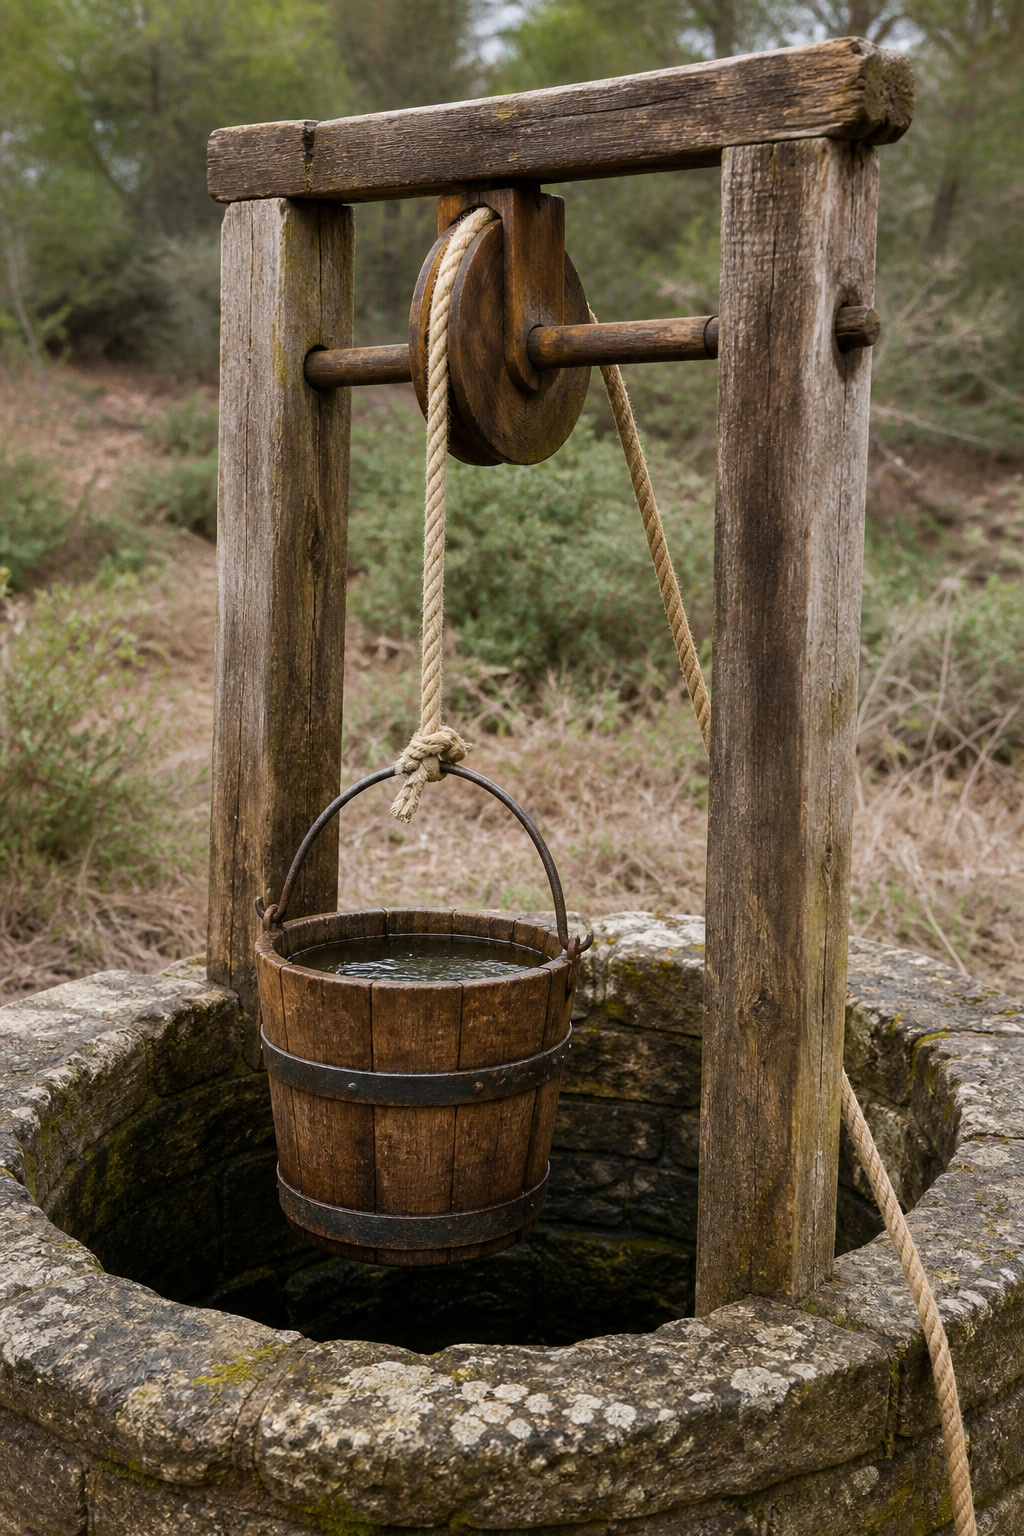
\includegraphics[width=0.34\linewidth]{images/book1/ai/g5-machines-pulley.jpg}

{\small De \omterm{def:g5:simple-machines:pulley}{katrol} van de put: het touw loopt in de groef, en een trek omlaag wordt een lift omhoog.}
\end{omfigure}

\begin{example}[Katrollen aan het werk]\label{ex:g5:simple-machines:pulleywork}
De vlag klimt langs de mast omhoog terwijl je handen comfortabel
\emph{omlaag} trekken: een vaste \omterm{def:g5:simple-machines:pulley}{katrol} bovenaan --- richting veranderd,
moeite gelijk, maar omlaag trekken laat je eigen \omterm{def:g4:weight-and-mass:weight}{gewicht} meehelpen. Het
takelblok van de bouwer schakelt meerdere katrollen zodat de last aan
vier of zes touwdelen hangt: elk deel draagt een kwart of een zesde
van het \omterm{def:g4:weight-and-mass:weight}{gewicht}, en één arbeider hijst een piano. Let wel op die
arbeider: \omterm{def:g2:measuring-length:units}{meter} na \omterm{def:g2:measuring-length:units}{meter} touw raast door zijn handen, terwijl de
piano traag omhoog kruipt.
\end{example}

\section{Het hellend vlak}

\begin{definition}[Hellend vlak]\label{def:g5:simple-machines:ramp}
Een \emph{hellend vlak}\index{hellend vlak} --- een helling --- is
een schuine baan om lasten omhoog te brengen zonder ze recht op te
tillen. Hoe flauwer de helling, hoe kleiner de duw die nodig is om de
last erlangs te bewegen: een vat een lange, flauwe helling op rollen
is makkelijk; een korte, steile helling op, moordend; recht omhoog,
onmogelijk.
\end{definition}

\begin{method}[Voel het met de elastiekunster]\label{met:g5:simple-machines:measure}
Je elastiekunster van vorig jaar proeft het verschil:
\begin{enumerate}
  \item laad een speelgoedautootje op een plank en haak het
        elastiekje eraan;
  \item zet de plank als flauwe helling op een laag stapeltje boeken;
        trek het autootje er langzaam aan het elastiekje op en noteer
        de rek;
  \item zet dezelfde plank veel steiler, op een stoelzitting, en trek
        opnieuw.
\end{enumerate}
De steile trek rekt het elastiekje veel verder uit: steilere helling,
grotere moeite. Flauwe hellingen zijn werkelijk flauw --- jouw
instrument zegt het.
\end{method}

\begin{omfigure}
\begin{tikzpicture}[scale=0.8]
  \draw[thick] (0,0) -- (11.2,0);
  \draw[very thick, omDef] (0.3,0) -- (6.5,2.0);
  \draw[thick, fill=omMeth, fill opacity=0.4]
    (2.8,0.82) rectangle ++(0.8,0.55);
  \draw[-Stealth, thick, omThm] (3.75,1.35) -- (4.65,1.64);
  \node[above, font=\small, omThm] at (3.4,1.75) {kleine duw};
  \draw[very thick, omDef] (8.2,0) -- (10.2,2.0);
  \draw[thick, fill=omMeth, fill opacity=0.4]
    (8.75,0.5) rectangle ++(0.8,0.55);
  \draw[-Stealth, very thick, omThm] (9.75,1.25) -- (10.55,2.05);
  \node[above, font=\small, omThm] at (9.3,1.9) {grote duw};
  \node[below, font=\small] at (3.4,-0.3)
    {lange flauwe helling naar dezelfde hoogte};
  \node[below, font=\small] at (9.3,-0.3) {korte steile helling};
\end{tikzpicture}

{\small Dezelfde kist, dezelfde hoogte te winnen: de lange flauwe
helling vraagt een kleine duw over een lange weg; de steile helling
een grote duw over een korte.}
\end{omfigure}

\begin{example}[Hellingen in het landschap]\label{ex:g5:simple-machines:ramps}
Rolstoelhellingen lopen lang en flauw naast korte trappen --- met
opzet zachtaardig. Bergwegen zigzaggen: in plaats van de top recht aan
te vallen, wikkelen ze een lang, flauw \omterm{def:g5:simple-machines:ramp}{hellend vlak} heen en weer over
de berghelling. En de schroef is een helling in vermomming --- een
schuine baan om een staafje gewikkeld, zodat elke makkelijke draai van
de schroevendraaier de schroef een piepklein stapje dieper laat
kruipen.
\end{example}

\section{De gulden regel}

\begin{proposition}[De gulden regel van de machines]\label{prop:g5:simple-machines:golden}
Geen enkele \omterm{def:g5:simple-machines:machine}{eenvoudige machine} geeft iets voor niets: wat ze aan
\omterm{def:g2:pushes-and-pulls:force}{kracht} bespaart, brengt ze in afstand in rekening. De helft van de
\omterm{def:g2:pushes-and-pulls:force}{kracht} --- twee keer zoveel touw binnenhalen, of twee keer zo'n lange
weg; een tiende van de \omterm{def:g2:pushes-and-pulls:force}{kracht} --- tien keer zo'n lange weg. Machine na
machine is de ruil exact: comfort koop je met \omterm{def:g2:measuring-length:units}{meters}.
\end{proposition}

\begin{example}[De regel controleren]\label{ex:g5:simple-machines:check}
De losse \omterm{def:g5:simple-machines:pulley}{katrol}: je hand trekt met de helft van de \omterm{def:g2:pushes-and-pulls:force}{kracht}, en om
de last \qty{1}{m} te laten stijgen haal je \qty{2}{m} touw binnen ---
beide touwdelen moeten een \omterm{def:g2:measuring-length:units}{meter} korter worden. De koevoet: jouw kant
veegt een lange boog, de zwerfkei verroert zich nauwelijks. De
helling: de kist bereikt dezelfde hoogte, maar je hebt hem de hele
schuine baan langs geduwd. Elke besparing precies betaald.
\end{example}

\begin{remark}[Waarom de regel niet te bedriegen is]\label{rem:g5:simple-machines:whygolden}
Onder de gulden regel schuilt onze oude bekende uit het
energiehoofdstuk: een last naar een hoogte tillen kost een vaste
portie \omterm{def:g5:everyday-energy:energy}{energie}, en geen enkele opstelling van touwen en planken
verandert die prijs. Machines laten je alleen in kleinere muntjes
betalen --- meer ervan. Een kleine \omterm{def:g2:pushes-and-pulls:force}{kracht} over een lange weg draagt
dezelfde \omterm{def:g5:everyday-energy:energy}{energie} over als een grote \omterm{def:g2:pushes-and-pulls:force}{kracht} over een korte. De
eeuwige machines mislukten om precies deze reden: de rekening blijft
de rekening.
\end{remark}

\section{Oefeningen}

\begin{exercise}[$\star$]\label{exo:g5:simple-machines:1}
Noem de drie klassieke \omterm{def:g5:simple-machines:machine}{eenvoudige machines}, en van elk één alledaagse
plek waar je haar vindt.
\end{exercise}

\begin{exercise}[$\star$]\label{exo:g5:simple-machines:2}
Wat verandert een vaste \omterm{def:g5:simple-machines:pulley}{katrol} aan jouw trek? En wat verandert een
losse \omterm{def:g5:simple-machines:pulley}{katrol}?
\end{exercise}

\begin{exercise}[$\star$]\label{exo:g5:simple-machines:3}
Waarom is een vlag omhoog hijsen door \emph{omlaag} te trekken
comfortabeler dan hetzelfde \omterm{def:g4:weight-and-mass:weight}{gewicht} recht optillen, terwijl de moeite
even groot is?
\end{exercise}

\begin{exercise}[$\star$]\label{exo:g5:simple-machines:4}
Met één losse \omterm{def:g5:simple-machines:pulley}{katrol} hangt de last aan twee touwdelen. Welk deel van
het \omterm{def:g4:weight-and-mass:weight}{gewicht} houdt jouw hand? Hoeveel touw moet je binnenhalen om de
last \qty{3}{m} te laten stijgen?
\end{exercise}

\begin{exercise}[$\star$]\label{exo:g5:simple-machines:5}
Welke helling rekt in \cref{met:g5:simple-machines:measure} het
elastiekje verder uit? Wat betaalt de kleinere rek van de flauwere
helling?
\end{exercise}

\begin{exercise}[$\star$]\label{exo:g5:simple-machines:6}
Waarom zigzaggen bergwegen in plaats van recht de helling op te lopen?
Welke \omterm{def:g5:simple-machines:machine}{eenvoudige machine} is de hele weg?
\end{exercise}

\begin{exercise}[$\star$]\label{exo:g5:simple-machines:7}
Formuleer de gulden regel van de machines. Een machine laat je met een
tiende van de \omterm{def:g2:pushes-and-pulls:force}{kracht} trekken --- wat brengt ze je in rekening?
\end{exercise}

\begin{exercise}[$\star$]\label{exo:g5:simple-machines:8}
Hoe is een schroef een \omterm{def:g5:simple-machines:ramp}{hellend vlak} in vermomming? Wat speelt de rol
van de lange flauwe weg?
\end{exercise}

\begin{exercise}[$\star\star$]\label{exo:g5:simple-machines:9}
Een takelblok laat een piano aan vier touwdelen hangen. Welk deel van
het \omterm{def:g4:weight-and-mass:weight}{gewicht} van de piano trekt de hand van de arbeider? Hoeveel
\omterm{def:g2:measuring-length:units}{meter} touw gaat er door zijn handen om de piano \qty{2}{m} te laten
stijgen?
\end{exercise}

\begin{exercise}[$\star\star$]\label{exo:g5:simple-machines:10}
Een laadhelling is \qty{6}{m} lang en stijgt \qty{1}{m}; een kist
erop duwen kost een bescheiden duw. De ongeduldige verhuizers zagen
een nieuwe helling van maar \qty{3}{m} lang naar hetzelfde platform.
Vergelijk met de gulden regel de nieuwe duw met de oude --- en leg uit
waarom ``de halve weg'' geen koopje was.
\end{exercise}

\begin{exercise}[$\star\star$]\label{exo:g5:simple-machines:11}
Een advertentie biedt een katrolset aan ``die zo slim is dat je één
\omterm{def:g2:measuring-length:units}{meter} touw met de helft van de \omterm{def:g2:pushes-and-pulls:force}{kracht} trekt --- en de last een hele
\omterm{def:g2:measuring-length:units}{meter} stijgt''. Zet de bewering voor het gerecht van de gulden regel
en de energierekening van \cref{rem:g5:simple-machines:whygolden}: zou
enige opstelling van wielen en touwen haar kunnen waarmaken?
\end{exercise}
